%----------------------------------------------------------------------------------------
%	PACKAGES AND THEMES
%----------------------------------------------------------------------------------------
\documentclass[aspectratio=169]{beamer}
\mode<presentation> {

	\usetheme{Boadilla}
}
\definecolor{lmugreen}{RGB}{0, 136, 58}
\usecolortheme[named=lmugreen]{structure}
\usepackage{graphicx} % Allows including images
\usepackage{booktabs} % Allows the use of \toprule, \midrule and \bottomrule in tables
\usepackage[english]{babel}
\usepackage[utf8]{inputenc}
\usepackage{amsmath,amssymb} % math symbols
\usepackage{graphicx}
\usepackage{float}
\usepackage{hyperref} % for URLs
\newcommand{\gray}{\rowcolor[gray]{.90}}
\usepackage{verbatim}
\usepackage{textpos} % logo position
\usepackage[default]{sourcesanspro} % font type
\usepackage{cases} % math cases
% Caption
\usepackage{caption}
\usepackage{tikz}
\usetikzlibrary{shapes.geometric, arrows.meta, positioning, fit, backgrounds}
\newcommand{\OnlineWorkflowMap}[5]{%
    \centering
    \scalebox{0.75}{%
    \begin{tikzpicture}[
        node distance=0.7cm and 0.8cm,
        box/.style={rectangle, draw, rounded corners, fill=blue!10,
                    text width=3cm, align=center, minimum height=1cm},
        database/.style={cylinder, draw, shape border rotate=90, aspect=0.25,
                    fill=orange!10, text width=2.6cm, align=center, minimum height=1.5cm},
        map focus/.style={draw=lmugreen, line width=1.8pt},
        arrow/.style={-{Stealth[scale=1.2]}, thick}
    ]
        \node (stream) [box, fill=green!10, #1]
            {Raw Data Stream\\(one pattern $x$ at a time)};

        \node (metric) [box, right=of stream, fill=purple!10, #2]
            {\textbf{Self-Adaptive Metric}\\ \textit{re-adjusted each round}};

        \node (compete) [box, right=of metric, text width=3.4cm, #3]
            {\textbf{Competition}\\ winner $s_1$ \& runner-up $s_2$\\ \textit{(2 nearest nodes)}};

        \node (update) [box, right=of compete, fill=yellow!20, text width=3.4cm, #4]
            {\textbf{Update Network}\\ absorb into $s_1$ \emph{or} new node\\ + reinforce edges};

        \node (net) [database, right=of update, #5]
            {\textbf{Self-Organizing}\\\textbf{Network}\\ nodes $V$ \& edges $E$};

        \begin{scope}[on background layer]
            \node [fit=(metric)(compete)(update), fill=blue!5, rounded corners,
                   draw, dashed,
                   label=above:\textbf{Online Phase (per pattern)}] {};
        \end{scope}

        \draw [arrow] (stream)  -- (metric);
        \draw [arrow] (metric)  -- (compete);
        \draw [arrow] (compete) -- (update);
        \draw [arrow] (update)  -- (net);
        \draw [arrow] (net.south) .. controls +(down:1.2cm) and +(down:1.2cm) ..
              node[midway, below, font=\scriptsize] {node positions $\rightarrow$ metric}
              (metric.south);
    \end{tikzpicture}
    }%
}
\newcommand{\MapFocus}{map focus}
\newcommand{\OnlineWorkflowFocusSlide}[5]{%
    \begin{frame}{Online Phase: #5}
        \OnlineWorkflowMap{#1}{#2}{#3}{#4}{}
    \end{frame}
}
\newcommand{\OnlineWorkflowNetworkFocusSlide}{%
    \begin{frame}{Online Phase: Self-Organizing Network}
        \OnlineWorkflowMap{}{}{}{\MapFocus}{\MapFocus}
    \end{frame}
}
\DeclareCaptionFont{tiny}{\tiny}
\captionsetup{font=scriptsize,labelfont=scriptsize,justification=centering}
% ToC
\AtBeginSection[]{
	\begin{frame}[noframenumbering, plain]
	\frametitle{Outline}
	\setcounter{tocdepth}{1}
	\tableofcontents[currentsection]
\end{frame}
}
% Remove navigation
\beamertemplatenavigationsymbolsempty
% R
\usepackage{listings}
\lstset{
language=R,
basicstyle=\scriptsize\ttfamily,
commentstyle=\ttfamily\color{gray},
backgroundcolor=\color{white},
showspaces=false,
showstringspaces=false,
showtabs=false,
tabsize=2,
captionpos=b,
breaklines=false,
breakatwhitespace=false,
title=\lstname,
escapeinside={},
keywordstyle={},
morekeywords={},
belowskip = -1.2 \baselineskip,
}
%----------------------------------------------------------------------------------------
%	TITLE PAGE
%----------------------------------------------------------------------------------------
\addtobeamertemplate{frametitle}{}{%
	\begin{textblock*}{100mm}(0.88\textwidth,-0.5cm)
		\includegraphics[height=1cm,width=2cm]{figures/lmu_logo}
\end{textblock*}}
\title{Practical Stream Clustering }
\author{Paul, Felix, Anton, Nils, Jack}
\institute[]{}
\date{13.07.2026}
\begin{document}
{
\usebackgroundtemplate{\includegraphics[width=\paperwidth]{figures/lmu-background.pdf}}
\begin{frame}
\begin{columns}
	\begin{column}{0.4\textwidth}
		\vspace{2cm}

		\textbf{\textcolor{white}{\Large LiarTree: Hierarchical Clustering for Real-Time Stream Data with Noise}}

		\textbf{\textcolor{white}{\large }}
		\vspace{1cm}

		\textcolor{white}{\footnotesize Paul Felkner, Felix Hajuj, Anton Hantschmann, Nils Hogenmüller, Shao-Chieh (Jack) Lien  \\
        \vspace{0.5cm}
			Mentors: Philipp Jahn, \\
            Dr. Gabriel Marques Tavares \\
			13.07.2026}
	\end{column}
	\begin{column}{0.57\textwidth}
		\vspace{1.56cm}
		\begin{center}
			\includegraphics[width=1\textwidth]{figures/lmu_grey.jpg}
		\end{center}
	\end{column}
\end{columns}
\end{frame}
}
%----------------------------------------------------------------------------------------
%	PRESENTATION SLIDES
%----------------------------------------------------------------------------------------



\section{Introduction \& Overview}

% ------------------------------------------------------------
% FRAME 1 — What is LiarTree?
% ------------------------------------------------------------
\begin{frame}{What is LiarTree?}

\end{frame}

% ============================================================
% FELIX — Task 2: Noise Handling
% ============================================================

% ------------------------------------------------------------
% FELIX 1 — Motivation
% ------------------------------------------------------------
\begin{frame}{Noise Handling: Motivation}
\begin{columns}[T]
  \begin{column}{0.55\textwidth}
    \textbf{Problem:} ClusTree inserts \emph{every} point into the nearest entry
    \begin{itemize}
      \item Real streams contain outliers and transient noise
      \item Noise inflates cluster radii and corrupts summaries
      \item No mechanism to separate signal from noise
    \end{itemize}
    \vspace{0.35cm}
    \textbf{LiarTree adds:}
    \begin{itemize}
      \item A per-node \emph{noise buffer} $\mathrm{CF}_\text{nb}$ (Def.\ 1)
      \item Suspected outliers are buffered, not inserted into entries
      \item Buffer graduates to a real cluster once evidence is sufficient
    \end{itemize}
  \end{column}
  \begin{column}{0.42\textwidth}
    \centering
    \vspace{0.5cm}
    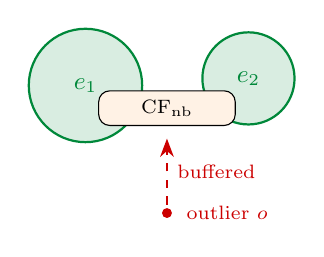
\begin{tikzpicture}[scale=0.9]
      % two cluster entries
      \draw[lmugreen, thick, fill=lmugreen!15] (-0.5,0.2) circle (0.8cm)
            node[font=\small]{$e_1$};
      \draw[lmugreen, thick, fill=lmugreen!15] (1.8,0.3) circle (0.65cm)
            node[font=\small]{$e_2$};
      % noise point
      \fill[red!80!black] (0.65,-1.6) circle (0.07cm);
      \node[red!80!black, font=\scriptsize] at (1.5,-1.6) {outlier $o$};
      % arrow to noise buffer box
      \draw[-{Stealth[scale=1.0]}, red!80!black, dashed, thick]
        (0.65,-1.48) -- (0.65,-0.55)
        node[midway, right, font=\scriptsize]{buffered};
      \node[draw, rounded corners, fill=orange!10, font=\scriptsize,
            text width=1.5cm, align=center] at (0.65,-0.12) {CF$_\text{nb}$};
    \end{tikzpicture}
  \end{column}
\end{columns}
\end{frame}

% ------------------------------------------------------------
% FELIX 2 — Noise Probability
% ------------------------------------------------------------
\begin{frame}{Noise Detection: Noise Probability (Def.\ 2)}
\begin{columns}[T]
  \begin{column}{0.56\textwidth}
    Score each arriving point against all entries at the current \textbf{inner} node:
    \[
      \mathrm{np}(o)
      \;=\;
      \min_{e \in \text{node}}\,\frac{\mathrm{dist}(o,\,\mu_e)}{r_e}
    \]
    \begin{itemize}
      \item $\mathrm{np}(o) < \theta$: inside some entry's radius $\;\Rightarrow\;$ insert normally
      \item $\mathrm{np}(o) \geq \theta$: far from all entries $\;\Rightarrow\;$ \textbf{buffer as noise}
    \end{itemize}
    \vspace{0.3cm}
    \textbf{Key design choice: check at inner nodes only}
    \begin{itemize}
      \item Leaf entries cover very few points $\to$ tiny, unstable radii
      \item Checking there would classify real data as noise
      \item Inner entries give a stable, subtree-wide view of the data
    \end{itemize}
  \end{column}
  \begin{column}{0.41\textwidth}
    \centering
    \vspace{0.5cm}
    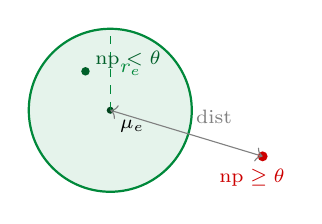
\begin{tikzpicture}[scale=0.9]
      % entry circle
      \draw[lmugreen, thick, fill=lmugreen!10] (0,0) circle (1.15cm);
      \fill[lmugreen!50!black] (0,0) circle (0.05cm);
      \node[font=\scriptsize, below right=0pt] at (0,0) {$\mu_e$};
      % radius label
      \draw[lmugreen, dashed]
        (0,0) -- (0,1.15) node[midway, right, font=\scriptsize]{$r_e$};
      % normal point (inside)
      \fill[lmugreen!70!black] (-0.35,0.55) circle (0.06cm);
      \node[lmugreen!70!black, font=\scriptsize] at (0.25,0.72) {$\mathrm{np}<\theta$};
      % noise point (outside)
      \fill[red!80!black] (2.15,-0.65) circle (0.07cm);
      \node[red!80!black, font=\scriptsize] at (2.0,-0.95) {$\mathrm{np}\geq\theta$};
      \draw[gray, thin, <->] (0,0) -- (2.15,-0.65)
            node[midway, above right, font=\scriptsize]{dist};
    \end{tikzpicture}
  \end{column}
\end{columns}
\end{frame}

% ------------------------------------------------------------
% FELIX 3 — Graduation
% ------------------------------------------------------------
\begin{frame}{Noise-to-Cluster Graduation (Def.\ 4)}
\textbf{Promotion test:}
$\quad g(n_\text{nb})\cdot\rho_\text{nb} \;\geq\; \rho_\text{avg}$
\quad only when \texttt{enc\_split = True}

\vspace{0.25cm}
\begin{columns}[T]
  \begin{column}{0.52\textwidth}
    \textbf{Gompertz gate} $\;g(n_\text{nb}) = e^{-b\,e^{-c\,n_\text{nb}}}$
    \begin{itemize}
      \item $g \approx 0$ for small buffers $\to$ no premature clusters
      \item $g \to 1$ once buffer size matches the average entry
      \item Anchored: $g(2)\approx 10^{-4}$,\ $g(n_\text{avg})\approx 0.97$
    \end{itemize}
    \vspace{0.2cm}
    \textbf{enc\_split flag} (set during tree descent)
    \begin{itemize}
      \item Triggered by a stale or empty entry anywhere on the path
      \item Signals concept drift: the tree has room to restructure
      \item Only then is introducing a new cluster appropriate
    \end{itemize}
  \end{column}
  \begin{column}{0.45\textwidth}
    \textbf{Implementation insight}\\[0.15cm]
    Noise probability reuses distances already computed by the overlap look-ahead
    $\;\Rightarrow\;$ \emph{zero extra distance calls}

    \vspace{0.35cm}
    \textbf{Interesting finding}\\[0.15cm]
    Overlap reduction keeps entries very dense, so the noise buffer rarely reaches $\rho_\text{avg}$
    --- the \emph{Echo Chamber} effect (see Eval.\ slides)

    \vspace{0.2cm}
    Fix: allow $\theta > 1$ to disable noise on clean datasets
  \end{column}
\end{columns}
\end{frame}

\section{Evaluation}

% ------------------------------------------------------------
% Evaluation Slide 1 — Methodology
% ------------------------------------------------------------
\begin{frame}{Parameter finetuning \& Evaluation: Methodology}
\begin{columns}[T]
\begin{column}{0.54\textwidth}
\begin{itemize}
    \item Approach: Bayesian Optimization (Optuna) + Parallel Programming (joblib)
    \item Performance: 12 datasets $\times$ 2 algorithms on 12 cores $\Rightarrow$ 40 min total; $\approx$ 2 min to find optimal parameters for each dataset
\end{itemize}
\end{column}
\begin{column}{0.44\textwidth}
\centering
\includegraphics[height=2.6cm]{figures/liartree_eval_p1}
\end{column}
\end{columns}
\vspace{0.3cm}
{\scriptsize
\begin{tabular}{p{0.18\linewidth}p{0.38\linewidth}p{0.38\linewidth}}
\toprule
\textbf{Method} & \textbf{Computational Cost} & \textbf{Optimality} \\
\midrule
Random Search & Medium (flexible) & Medium (good coverage but may miss best regions) \\
Multi-stage Grid Search & High (repeated structured grid evaluations, even if refined) & High (progressive refinement increases chance of near-optimal solution) \\
Bayesian Optimization & Low: few evaluations needed due to guided search & Very high: typically near-optimal under limited budget \\
\bottomrule
\end{tabular}
}
\end{frame}

% ------------------------------------------------------------
% Evaluation Slide 2 — Evaluated data
% ------------------------------------------------------------
\begin{frame}{Parameter finetuning \& Evaluation: Evaluated data}
\begin{itemize}
    \item Algorithm: ClusTree, LiarTree
    \item Dataset: (Complex9, Stream\_Densired) $\times$ 6 noise levels (0\%, 10\%, 20\%, 30\%, 40\%, 50\%)
    \item Tunable parameters
    \begin{itemize}
        \item ClusTree: online: $\lambda$ decay ($0.00001$--$4$). offline: $\epsilon$ ($0.005$--$0.5$), minSamples ($1$--$20$)
        \item LiarTree: online: $\lambda$ decay ($0.00001$--$4$), noise threshold ($0$--$1$), offline: $\epsilon$ ($0.005$--$0.5$), minSamples ($1$--$20$)
    \end{itemize}
    \item Unlimited budget
\end{itemize}
\end{frame}

% ------------------------------------------------------------
% Evaluation Slide 3 — Result
% ------------------------------------------------------------
\begin{frame}{Parameter finetuning \& Evaluation: Result}
\vspace{0.4cm}
\begin{center}
\includegraphics[width=0.7\linewidth]{figures/liartree_eval_p3-1}\hspace{0.3cm}%
\includegraphics[width=0.23\linewidth]{figures/liartree_eval_p3-3}\\[0.3cm]
\includegraphics[width=0.7\linewidth]{figures/liartree_eval_p3-2}\hspace{0.3cm}%
\includegraphics[width=0.23\linewidth]{figures/liartree_eval_p3-4}
\end{center}
\end{frame}

% ------------------------------------------------------------
% Evaluation Slide 4 — Root Cause Analysis (Echo Chamber I)
% ------------------------------------------------------------
\begin{frame}{Root Cause Analysis: Echo Chamber effect}
\begin{itemize}
    \item ClusTree strives to make radius smaller
    \begin{itemize}
        \item Local Look-Ahead
        \item Variance Reduction for Noise to Cluster event
    \end{itemize}
    \item Strict noise-to-buffer criteria
    \begin{itemize}
        \item Noise buffer's accumulated density needs to exceed the average density of regular entries
    \end{itemize}
    \item Combined effect
    \begin{itemize}
        \item Few points enter the entries and they remain always dense
        \item Arriving data density stays constant: noise buffer never gets dense enough
    \end{itemize}
    \item Applies to larger data (covtype: $\sim$600,000) and concept drift data (stream\_densired)
\end{itemize}
\end{frame}

% ------------------------------------------------------------
% Evaluation Slide 5 — Root Cause Analysis (Echo Chamber II)
% ------------------------------------------------------------
\begin{frame}{Root Cause Analysis: Echo Chamber effect}
\begin{itemize}
    \item Solution: Lower the density threshold for the noise-to-cluster process
    \item Mitigation: Set noise threshold to $0$--$1.5$ during param finetuning ($>1$: disable noise)
\end{itemize}
\vspace{0.4cm}
\begin{center}
\includegraphics[width=0.5\linewidth]{figures/liartree_eval_p5-1}\hfill
\includegraphics[width=0.5\linewidth]{figures/liartree_eval_p5-2}
\end{center}
\end{frame}

% ------------------------------------------------------------
% Evaluation Slide 6 — Result with disableable noise threshold
% ------------------------------------------------------------
\begin{frame}{Parameter finetuning \& Evaluation: Result with disableable noise threshold}
\begin{itemize}
    \item No obvious superiority of LiarTree
    \item However, the finetuning objective function (current: cmm $\times$ f1) may result in different performance
\end{itemize}
\vspace{0.2cm}
\begin{center}
\includegraphics[height=2.5cm]{figures/liartree_eval_p6-1}\hspace{0.3cm}%
\includegraphics[height=2.5cm]{figures/liartree_eval_p6-3}\\[0.15cm]
\includegraphics[height=2.5cm]{figures/liartree_eval_p6-2}\hspace{0.3cm}%
\includegraphics[height=2.5cm]{figures/liartree_eval_p3-4}
\end{center}
\end{frame}

% ------------------------------------------------------------
% Evaluation Slide 7 — Anytime Evaluation: Methodology
% ------------------------------------------------------------
\begin{frame}{Anytime Evaluation: Methodology}
\begin{itemize}
    \item ON/OFF Burst Traffic Model
    \begin{itemize}
        \item Pros: Captures real-world burstiness; good for stress testing
        \item Cons: Oversimplified; lacks smooth transitions (doesn't reflect gradual load changes)
    \end{itemize}
    \item Sinusoidal
    \begin{itemize}
        \item Pros: Easy to tune; useful for periodic workloads (e.g., daily usage patterns)
        \item Cons: Unrealistic for bursty traffic; can mask worst-case behavior
    \end{itemize}
    \item Live Traffic
    \begin{itemize}
        \item Pros: Most realistic evaluation
        \item Cons: Hard to reproduce/debug; expensive to collect and use
    \end{itemize}
\end{itemize}
\end{frame}

% ------------------------------------------------------------
% Evaluation Slide 8 — Anytime Evaluation: Result
% ------------------------------------------------------------
\begin{frame}{Anytime Evaluation: Result}
\begin{itemize}
    \item ClusTree: $\lambda = 0.001454$, $\epsilon = 0.024218$, minSamples $= 1$
    \item LiarTree: $\lambda = 0.246025$, noise threshold $= 1.160854$, $\epsilon = 0.022021$, minSamples $= 6$
\end{itemize}
\vspace{0.2cm}
\begin{center}
\includegraphics[height=2.5cm]{figures/liartree_eval_p8-1}\hspace{0.3cm}%
\includegraphics[height=2.5cm]{figures/liartree_eval_p8-3}\\[0.15cm]
\includegraphics[height=2.5cm]{figures/liartree_eval_p8-2}\hspace{0.3cm}%
\includegraphics[height=2.5cm]{figures/liartree_eval_p8-4}
\end{center}
\end{frame}

% ------------------------------------------------------------
% Evaluation Slide 9 — Anytime Evaluation: Root Cause Analysis
% ------------------------------------------------------------
\begin{frame}{Anytime Evaluation: Root Cause Analysis}
\begin{itemize}
    \item LiarTree requires 3x more budget than ClusTree
    \item LiarTree accumulated much more points in buffer during data burst
    \item Hitchhiker has a much larger radius when it is carried to leaf
\end{itemize}
\vspace{0.2cm}
\begin{center}
\begin{minipage}[t]{0.32\linewidth}
\centering
\includegraphics[height=3.3cm]{figures/liartree_eval_p9-2}\\[0.1cm]
{\scriptsize ClusTree (freq=3, mag=0.6)}
\end{minipage}\hfill
\begin{minipage}[t]{0.32\linewidth}
\centering
\includegraphics[height=3.3cm]{figures/liartree_eval_p9-1}\\[0.1cm]
{\scriptsize LiarTree (freq=3, mag=0.6)}
\end{minipage}\hfill
\begin{minipage}[t]{0.32\linewidth}
\centering
\includegraphics[height=3.3cm]{figures/liartree_eval_p9-3}
\end{minipage}
\end{center}
\end{frame}

% ------------------------------------------------------------
% Evaluation Slide 10 — Visualization
% ------------------------------------------------------------
\begin{frame}{Visualization: Anytime in action}
\begin{center}
\includegraphics[width=0.72\linewidth]{figures/liartree_eval_p10}
\end{center}
\end{frame}

% ------------------------------------------------------------
% Evaluation Last Slide — References
% ------------------------------------------------------------
\begin{frame}{References}
\begin{itemize}
    \item Param finetuning strategy: \url{https://medium.com/@mdshah930/a-practical-guide-to-hyperparameter-tuning-grid-search-random-search-bayesian-optimization-f0946fbcbbc6}
\end{itemize}
\end{frame}

\section{Appendix}


\end{document}
